% CP11: geometric reconstruction of FIG 14.6 from author scan F14_6.jpg.
% Pixel coordinates used below reproduce VISIBLE PRINTED INK only, not atomic potential data.
% Scientific provenance: Akulin--Karlov R36, lecture 14, caption Fig 14.6.
% Interpret E as the common vertical energy axis and Gamma(E) as the left density plot.
\documentclass[border=6pt]{standalone}
\usepackage{fontspec,unicode-math}
\setmainfont{Noto Serif}
\setmathfont{STIXTwoMath-Regular.otf}
\usepackage{tikz}
\usetikzlibrary{arrows.meta,patterns}
\tikzset{pot/.style={line width=1.18pt,line cap=round,line join=round},
 level/.style={line width=.8pt}, density/.style={line width=.7pt},
 axis/.style={line width=.56pt,-{Latex[length=2mm,width=1.15mm]}},
 release/.style={line width=.63pt,-{Latex[length=1.85mm,width=.98mm]}},
 guide/.style={line width=.55pt,densely dashed},
 lab/.style={font=\fontsize{12}{14}\selectfont,inner sep=1.2pt},
 little/.style={font=\fontsize{10.2}{12}\selectfont,inner sep=1pt}}
\begin{document}
% Positive downward pixel-Y is accounted for by y=-0.013cm.
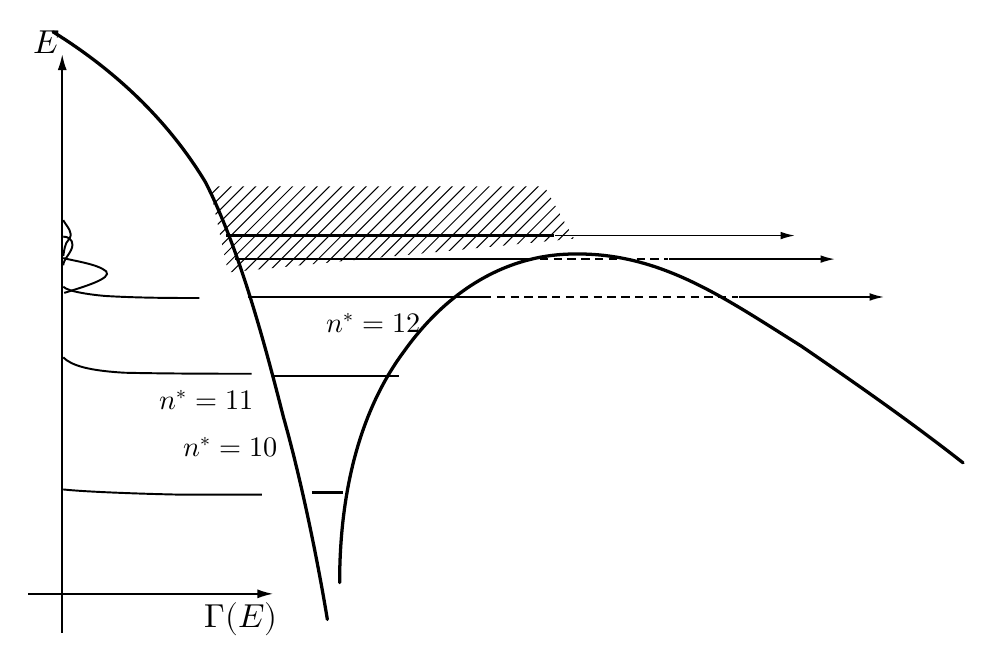
\begin{tikzpicture}[x=.013cm,y=-.013cm]
% Common E axis and horizontal Gamma(E) axis in source, not an independent panel.
\draw[axis] (40,597)--(40,32);
\node[lab,anchor=south east] at (40,35) {$E$};
\draw[axis] (7,559)--(246,559);
\node[lab,anchor=north] at (215,564) {$\Gamma(E)$};
% Printed left-hand spectral line density: deliberately qualitative and without calibrated ordinate.
\draw[density] (41,194).. controls (45,201) and (51,206) .. (47,212)
 .. controls (42,217) and (42,224) .. (41,229);
\draw[density] (41,210).. controls (46,210) and (50,213)..(50,218)
 .. controls (50,225) and (41,232)..(41,238);
\draw[density] (41,231)..controls (53,234) and (75,237).. (83,244)
 ..controls (89,251) and (61,259) .. (42,265);
\draw[density] (41,259)..controls (46,264) and (70,267)..(82,268)
 ..controls (115,270) and (150,270)..(174,270);
\draw[density] (41,328)..controls (49,336) and (66,341).. (101,343)
 .. controls (145,344) and (203,344)..(225,344);
\draw[density] (41,457)..controls (58,459) and (106,461).. (151,462)
 .. controls (186,462) and (220,462)..(235,462);
% Statically anchored potential traces. No speculative numerical eigenfunctions.
\draw[pot] (31,10) .. controls (89,46) and (142,94) .. (180,157)
 .. controls (211,218) and (235,303) .. (256,386)
 .. controls (275,453) and (291,535) .. (299,584);
\draw[pot] (311,548) .. controls (311,461) and (330,381) .. (374,322)
 .. controls (416,263) and (474,227) .. (541,227)
 .. controls (625,226) and (687,270) .. (762,317)
 .. controls (816,354) and (869,391) .. (920,431);
% Original upper hatched region: graphical continuum, not measured band.
\begin{scope}
 \clip (184,161)--(511,161)--(540,212)--(202,245)--cycle;
 \foreach \t in {0,12,...,900}{\draw[line width=.37pt] (\t,150)--(\t-102,252);}
\end{scope}
% Horizontal levels inside the well, with widths from the author scan.
\draw[level] (284,460)--(314,460);
\node[little,anchor=east] at (254,416) {$n^*=10$};
\draw[level] (246,346)--(369,346);
\node[little,anchor=east] at (230,370) {$n^*=11$};
\draw[level] (221,269)--(451,269);
\node[little,anchor=north] at (344,282) {$n^*=12$};
\draw[level] (209,232)--(493,232);
\draw[level] (200,209)--(520,209);
% Escape directions and dashed tunnelling/continuum guide sections.
\draw[guide] (493,232)--(632,232);\draw[release] (633,232)--(795,232);
\draw[guide] (451,269)--(700,269);\draw[release] (701,269)--(843,269);
\draw[release] (521,209)--(756,209);
\end{tikzpicture}
\end{document}
